\documentclass[11pt]{article}

\usepackage[fleqn]{amsmath}
\usepackage{amssymb}
\usepackage[english]{babel}
\usepackage{bookmark}
\usepackage{booktabs}
\usepackage{capt-of}
\usepackage{colortbl}
\usepackage{dcolumn}
\usepackage{fancyhdr}
\usepackage[T1]{fontenc}
\usepackage{graphicx}
\usepackage{grffile}
\usepackage{hyperref}
\usepackage[utf8]{inputenc}
\usepackage{listings}
\usepackage{longtable}
\usepackage{rotating}
\usepackage{textcomp}
\usepackage{tikz}
\usepackage[normalem]{ulem}
\usepackage{verbatim}
\usepackage{wrapfig}
\usepackage{xeCJK}

\usetikzlibrary{mindmap,trees}

\newcommand{\rmnum}[1]{\romannumeral #1}
\newcommand{\HRule}{\rule{\linewidth}{0.5mm}}
\newcommand{\Rmnum}[1]{\expandafter\@slowromancap\romannumeral #1@}
\setCJKmonofont{PingFang SC}
\setCJKmainfont{PingFang SC}
\setsansfont{GoMono Nerd Font}
\setmainfont{GoMono Nerd Font}
\setmonofont[Mapping={}]{GoMono Nerd Font}
\lstset{
  breaklines=true,
  breakatwhitespace=false,
  captionpos=b,
  tabsize=2,
  numbers=left,
  numberstyle=\tiny\color{gray},
  columns=fullflexible,
  frame=shadowbox,
  keepspaces=true,
  commentstyle=\color[RGB]{0,128,0},
  keywordstyle=\color[RGB]{0,0,255},
  basicstyle=\footnotesize\ttfamily,
  rulesepcolor=\color{red!20!green!20!blue!20},
  showstringspaces = false,
}

\graphicspath{{figures/}}
\allowdisplaybreaks

\setcounter{page}{1}

\begin{document}

\begin{center}
  \textbf{\Huge{第四章作业}}
\end{center}

\section*{4.47}

\subsection*{A}
\begin{lstlisting}[language=c]
#include <stdio.h>

void bubble(long *data , long count) {
  long *i, *last;
  for (last = data + count - 1; last > data; --last)
    for (i = data; i < last; ++i)
      if (*(i + 1) < *i) {
        long t = *(i + 1);
        *(i + 1) = *i;
        *i = t;
      }
}

int main() {
  long a[4] = {4, 2, 3, 1};
  bubble(a, 4);
  for (int i = 0; i < 4; ++i) printf("%ld ", a[i]);
  return 0;
}
\end{lstlisting}

\subsection*{B}
由于Y86-64中无乘法和leaq指令,所以bubble函数改为传入两个指针begin和end,表示数组
的头和尾(均被包含在数组中)。
\begin{lstlisting}[language={[x86masm]Assembler}]
.pos 0
  irmovq stack, %rsp
  call main
  halt

# Array of 4 elements
.align 8
begin:
  .quad 0x0000000000000002
  .quad 0x0000000000000004
  .quad 0x0000000000000001
end:
  .quad 0x0000000000000003

main:
  irmovq begin, %rdi
  irmovq end, %rsi
  call bubble
  ret

# void bubble(long *begin, long *end)
# begin in %rdi, end in %rsi
bubble:
  jmp L2
L4:
  mrmovq 8(%rax), %r9
  mrmovq (%rax), %r10
  rrmovq %r9, %r8
  subq %r10, %r8
  jge L3
  rmmovq %r10, 8(%rax)
  rmmovq %r9, (%rax)
L3:
  irmovq $8, %r8
  addq %r8, %rax
  jmp L5
L6:
  rrmovq %rdi, %rax
L5:
  rrmovq %rsi, %r8
  subq %rax, %r8
  jg L4
  irmovq $8, %r8
  subq %r8, %rsi
L2:
  rrmovq %rsi, %r8
  subq %rdi, %r8
  jg L6
	ret

  
.pos 0x200
stack:
\end{lstlisting}

\begin{figure*}[htbp!]
  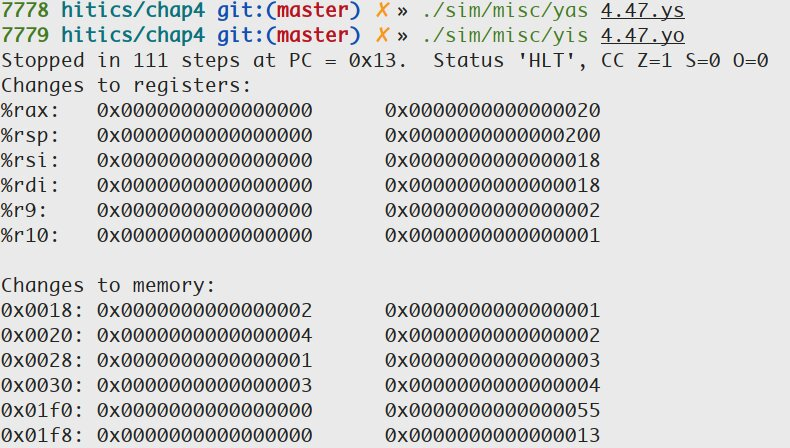
\includegraphics[width=\linewidth]{figures/4.47.jpg}
  \caption{运行结果}
\end{figure*}

\section*{4.51}
\begin{tabular}[htbp!]{|c|l|}
  \hline
  阶段 & $ iaddq\ \mathbf{V,\ rB} $ \\
  \hline
  取值 & $ icode:ifun \leftarrow M_1[PC] $ \\
       & $ rA:rB \leftarrow M_1[PC] $ \\
       & $ valC \leftarrow M_8[PC + 2] $ \\
       & $ valP \leftarrow PC + 10 $ \\
  \hline
  译码 & $ valB \leftarrow R[rB] $ \\
  \hline
  执行 & $ valE \leftarrow valB + valC $ \\
       & $ Set\ CC $ \\
  \hline
  访问 & \\
  \hline
  写回 & $ R[rB] \leftarrow valE $ \\
  \hline
  更新 $ PC $ & $ PC \leftarrow valP $ \\
  \hline
\end{tabular}

\section*{4.59}

4.47的版本最优。\\\\
4.47版本中的循环部分如下:
\begin{lstlisting}[language={[x86masm]Assembler}]
L4:
  mrmovq 8(%rax), %r9
  mrmovq (%rax), %r10
  rrmovq %r9, %r8
  subq %r10, %r8
  jge L3
  rmmovq %r10, 8(%rax)
  rmmovq %r9, (%rax)
\end{lstlisting}
单个循环最多有7条指令。\\\\
4.48版本中的循环部分如下:
\begin{lstlisting}[language={[x86masm]Assembler}]
L4:
  mrmovq 8(%rax), %r9
  mrmovq (%rax), %r10
  rrmovq %r9, %r8
  subq %r10, %r8
  cmovl %r9, %r11
  cmovl %r10, %r9
  cmovl %r11, %r10
  rmmovq %r9, 8(%rax)
  rmmovq %r10, (%rax)
\end{lstlisting}
单个循环最多有9条指令。\\\\
4.49版本中的循环部分如下:
\begin{lstlisting}[language={[x86masm]Assembler}]
L4:
  mrmovq 8(%rax), %r9
  mrmovq (%rax), %r10
  rrmovq %r9, %r8
  rrmovq %r10, %r11
  xorq %r9, %r10
  subq %r11, %r8
  cmovge %r11, %r9
  xorq %r10, %r9
  xorq %r9, %r10
  rmmovq %r9, 8(%rax)
  rmmovq %r10, (%rax)
\end{lstlisting}
单个循环最多有11条指令。\\\\
4.47的版本的指令最少,单次循环耗时较少。

\end{document}
